\documentclass{article}

\usepackage[utf8]{inputenc}
\usepackage{amsmath}
\usepackage{graphicx}
\usepackage{geometry}
\usepackage{float}
\usepackage{hyperref}
\usepackage{subcaption}

% Adjust the page margins
\geometry{a4paper, margin=1in}

\begin{document}

\begin{titlepage}
    \centering
    % Title centered in the middle of the page
    \vspace*{9cm} % Adjust the vertical space for title placement
    {\Huge \textbf{Population Density Insights for Sindh}\par}
    \vspace{0.5cm}
    % Subtitle
    {\Large Findings from the Pakistan Census 2023\par}
    
    % Author and Date at the bottom center
    \vfill
    {\Large Muhammad Azeem Haider\par}
    \vspace{0.5cm}
    {\Large \today\par}
\end{titlepage}

\section*{Introduction}
This document presents an analysis of Sindh's population across its districts, based on data from the Pakistan Census 2023, which provides insights into population, housing, literacy, and other key indicators.

\vspace{0.5cm}

\noindent The analysis addresses two key questions:

\begin{enumerate}
    \item Comparison of land and population ratios across Sindh's districts.
    \item Identification of districts where the average household size exceeds the provincial average.
\end{enumerate}

\noindent According to a United Nations report, the global population is expected to reach approximately 9.7 billion by 2050, with a further increase to 11.2 billion by 2100. Pakistan is projected to be one of the most populous countries, ranking fourth after India, China, and the United States.

\begin{figure}[H]
    \centering
    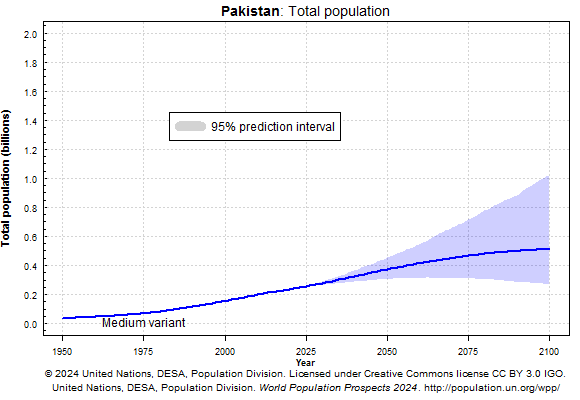
\includegraphics[width=\textwidth]{../Figures/Figure01.png}
    \caption{Projected population growth of Pakistan according to the United Nations.}
    \label{fig:fig1}
\end{figure}

\noindent Figure \ref{fig:fig1} illustrates the projected population growth of Pakistan, which will impact population distribution across its provinces. The information is prediction carried out by the Population Division of the Department of Economic and Social Affairs of the United Nations Secretariat \cite{bib01}.

\vspace{0.5cm}

\noindent The 2023 population census provides valuable information on this distribution. The report from the Pakistan census of 2023 is used as a guiding source \cite{bib02}. The data is analyzed to understand the population distribution across Sindh's districts and identify areas with higher population densities.

\begin{center}
    \begin{tabular}{ |p{3cm}|p{3cm}|p{3cm}|p{3cm}|p{3cm}|  }
        \hline
        \multicolumn{5}{|c|}{Percentage Population Distribution in Different Provinces of Pakistan in Census 2023} \\ 
        \hline
        Balochistan & Sindh & Punjab & Khyber Pakhtunkhwa & Islamabad \\ 
        \hline
        6.2\% & 23.1\% & 52.9\% & 16.9\% & 1.0\% \\ 
        \hline
    \end{tabular}
\end{center}

\noindent Table above shows the percentage distribution of the population across Pakistan's provinces. Sindh, with 23.1\%, has the second-highest population, and its share has steadily increased since the 1961 census. In contrast, other provinces like Balochistan, Punjab, and Khyber Pakhtunkhwa have either fluctuated or seen declines in their population shares.

\begin{figure}[H]
    \centering
    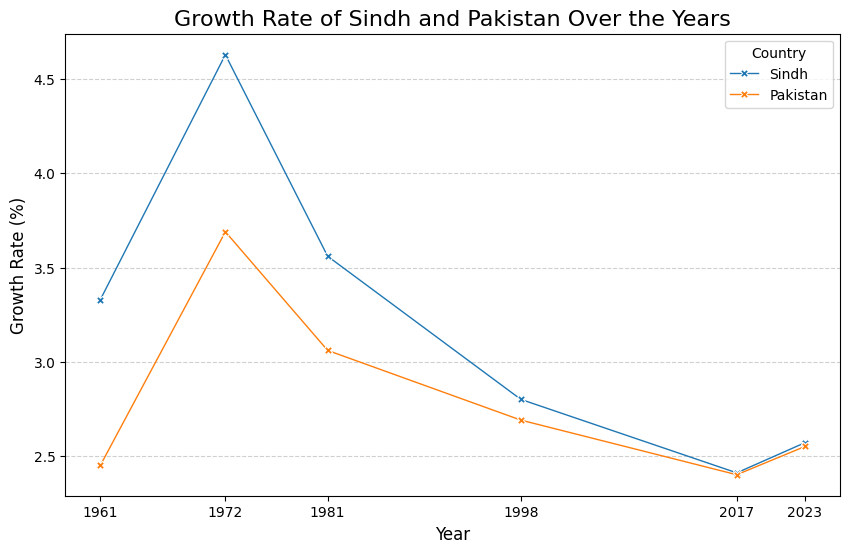
\includegraphics[width=\textwidth]{../Figures/Figure02.png}
    \caption{Population growth trends in Sindh and Pakistan across different censuses.}
    \label{fig:fig2}
\end{figure}

\noindent Figure \ref{fig:fig2} compares the population growth of Sindh and Pakistan across censuses. Historically, Sindh's population growth has been higher than the national average, with the largest gap of 0.94\% observed in 1972. However, this difference has decreased over time, with the 2023 census showing only a 0.02\% difference. This difference was reduced to 0.01\% in the census of 2017. This means that the population growth of Sindh and Pakistan is almost the same since 2017. 

\section*{Analysis}
\noindent Sindh is the second biggest province of Pakistan in terms of population. The province is constantly growing its share of total population in Pakistan. According to the Pakistan census of 2023, Sindh has 30 districts. The land mass of Sindh has 17.70\% of the total land of Pakistan. The unequal population distribution in Pakistan is evident from the fact that Balochistan, province with the most landmass, has the lowest population share of 6.2\% in the country. 

\vspace{0.5cm}

\noindent Figure \ref{fig:fig3} shows the percentage of landmass of the four provinces and the federal capital, Islamabad, of Pakistan. The highest population share of Pakistan is carried out by Pakistan standing at 52.9\%. It is interesting that higher landmass does not equal high population. This unequal distribution of population can ultimately be explained by the number opportunities present in the province, security, and safety of the province. Since this document focuses on Sindh, it is important to analyze if similar patterns arise in the Sindh province, where unequal distribution of population can be seen mainly because of the opportunities present in the district. 

\begin{figure}[H]
    \centering
    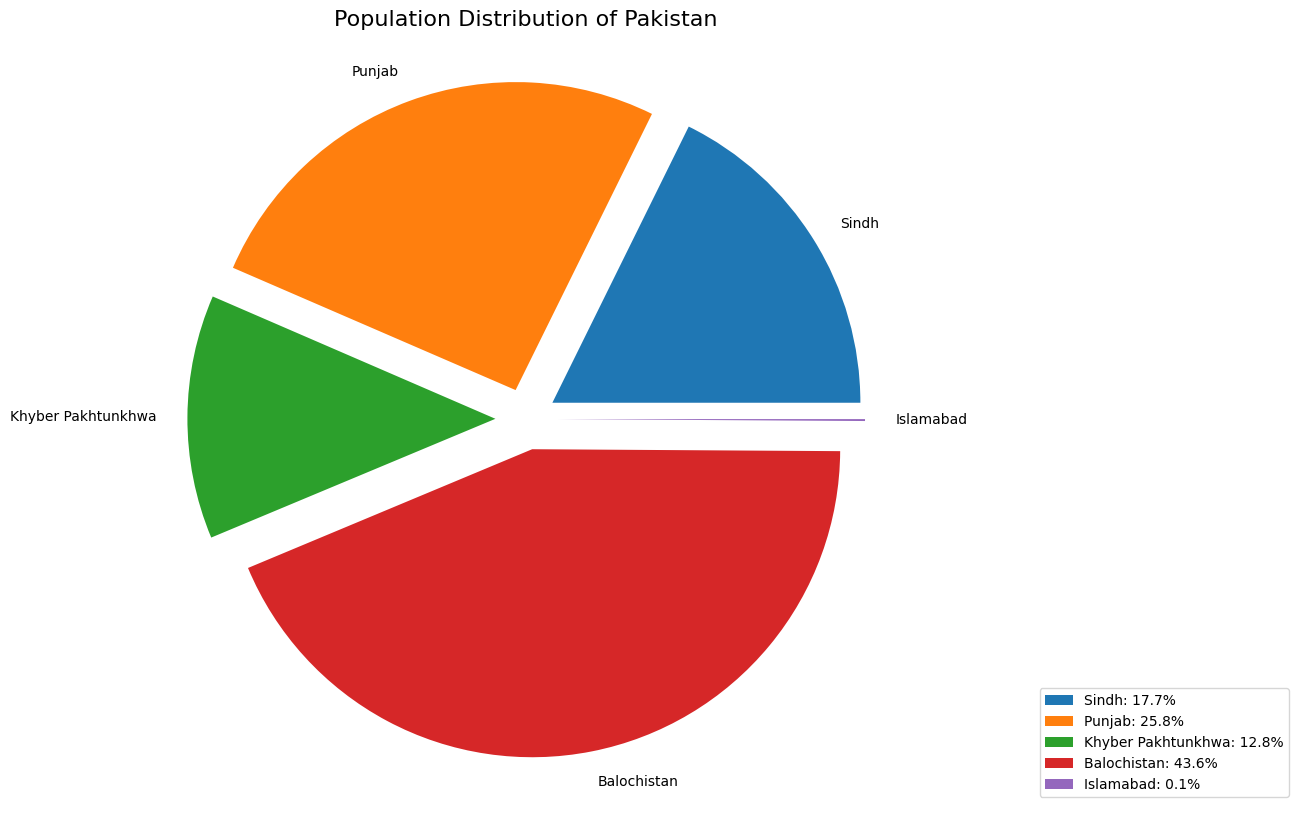
\includegraphics[width=\textwidth]{../Figures/Figure03.png}
    \caption{Percentage of Population landmass across Sindh's districts.}
    \label{fig:fig3}
\end{figure}

\noindent The population of Sindh is divided into 30 districts. However, this population is not divided equally amongst districts. The highest population density is observed in the seven sub-districts of Karachi. 

\vspace{0.5cm}

\begin{figure}[H]
    \centering
    \begin{subfigure}[b]{0.45\textwidth}
        \centering
        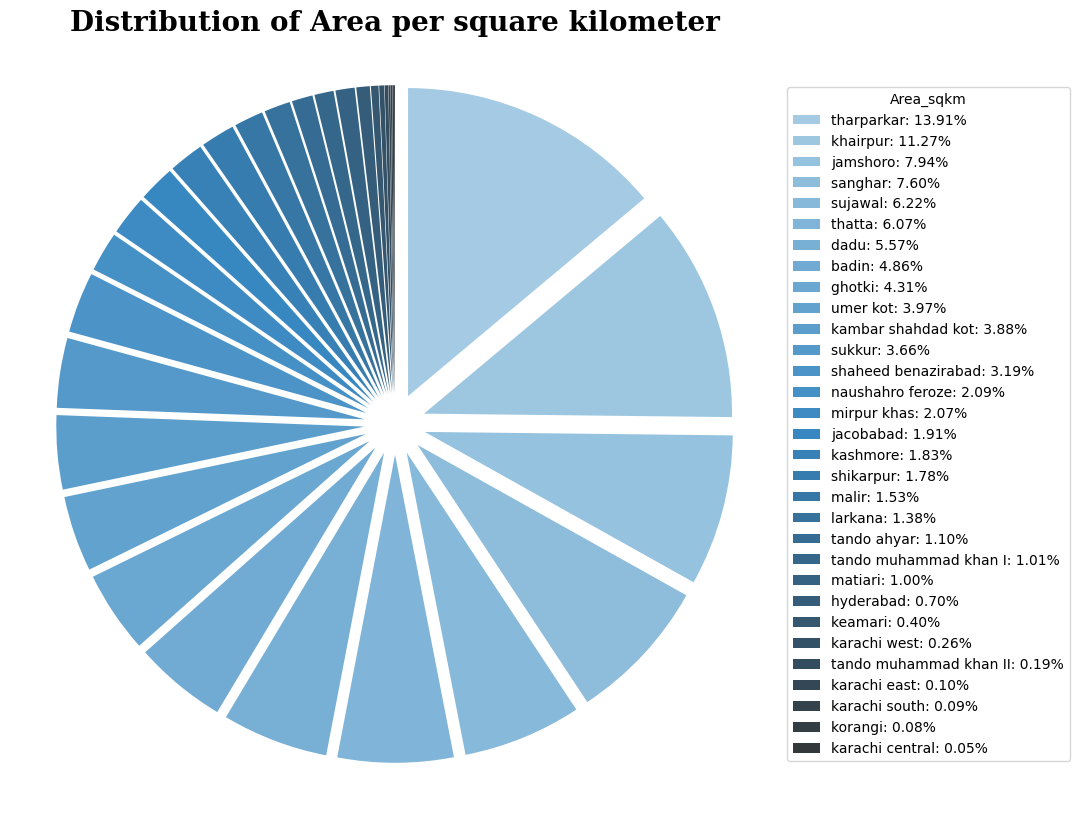
\includegraphics[width=\textwidth]{../Figures/Figure04.png}
        \caption{Percentage landmass of different districts of Sindh.}
        \label{fig:fig4a}
    \end{subfigure}
    \hfill
    \begin{subfigure}[b]{0.45\textwidth}
        \centering
        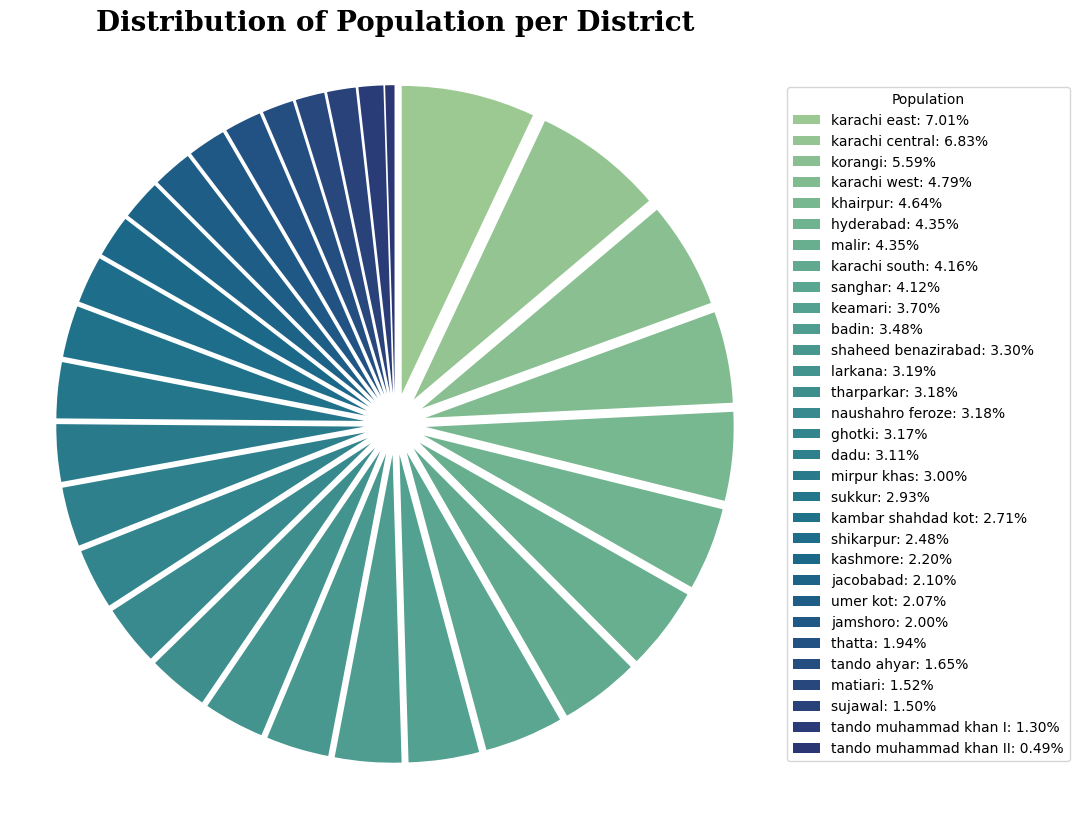
\includegraphics[width=\textwidth]{../Figures/Figure05.png}
        \caption{Distribution of population across different districts of Sindh.}
        \label{fig:fig4b}
    \end{subfigure}
    \caption{Comparison of different districts of Sindh on the basis of landmass and population.}
    \label{fig:fig4}
\end{figure}

\noindent Tharparkar is the largest district in Sindh with a landmass ratio of 13.91\% of the total land of Sindh, however it has a low population density ratio with only accounting to 3.18\% of the total population of Sindh. In contrast, six out of the seven lowest districts in terms of landmass comes from Karachi, with Malir, the seventh sub-district of Karachi having the highest landmass ratio of 1.53\% of the total land of Sindh. Adding up the landmass of the seven sub-districts of Karachi, the total landmass of Karachi comes out to be 2.51\% of the total land of Sindh. In contrast, the population of Karachi equates to a staggering 36.43\% of the total population of Sindh.

\vspace{0.5cm}

\noindent This inequality in landmass and population can be seen in figure \ref{fig:fig4}. Figure \ref{fig:fig4a} shows the distribution of landmass across different districts of Sindh, whereas, figure \ref{fig:fig4b} shows the distribution of population across different districts of Sindh.

\vspace{0.5cm}

\noindent It is important to understand why this inequality in population density exists to the point where more than $\frac{1}{3}$rd of the population of the province resides in one city which is only 1.53\% of the total landmass of the province. This can be attributed to many factors, which includes economic opportunities, better living standards, and better infrastructure. Karachi is considered the economic hub of the country by contributing a major chunk of the country's GDP and overall tax revenue. As of 2015, according to an economic and financial analysis report by Asian development bank \cite{bib3}, Karachi is estimated to represent 25\% of the national GDP and contributes to 35\% of the countrys tax revenue. 

\vspace{0.5cm}

\noindent The average household size of the Sindh province is 5.53. This means that on average, every family in the Sindh province have approximately 6 members. 13 out of 30 districts of Sindh have the average household size higher than the average household size of the province. The following districts have the average household size greater. 

\begin{itemize}
    \item Jacobabad, Kambar Shahdad Kot, Karachi Central, Karachi East, Karachi West, Kashmore, Keamari, Khairpur, Korangi, Malir, Sanghar, Shikarpur, Sukkur
\end{itemize}

\noindent Karachi being the economic hub of the province and the country means it has better housing infrastructure. The population census of 2023 divides the housing infrastructure into three categories, namely:

\begin{itemize}
    \item Pakka, Semi-Pakka, Kacha
\end{itemize}

\begin{figure}[H]
    \centering
    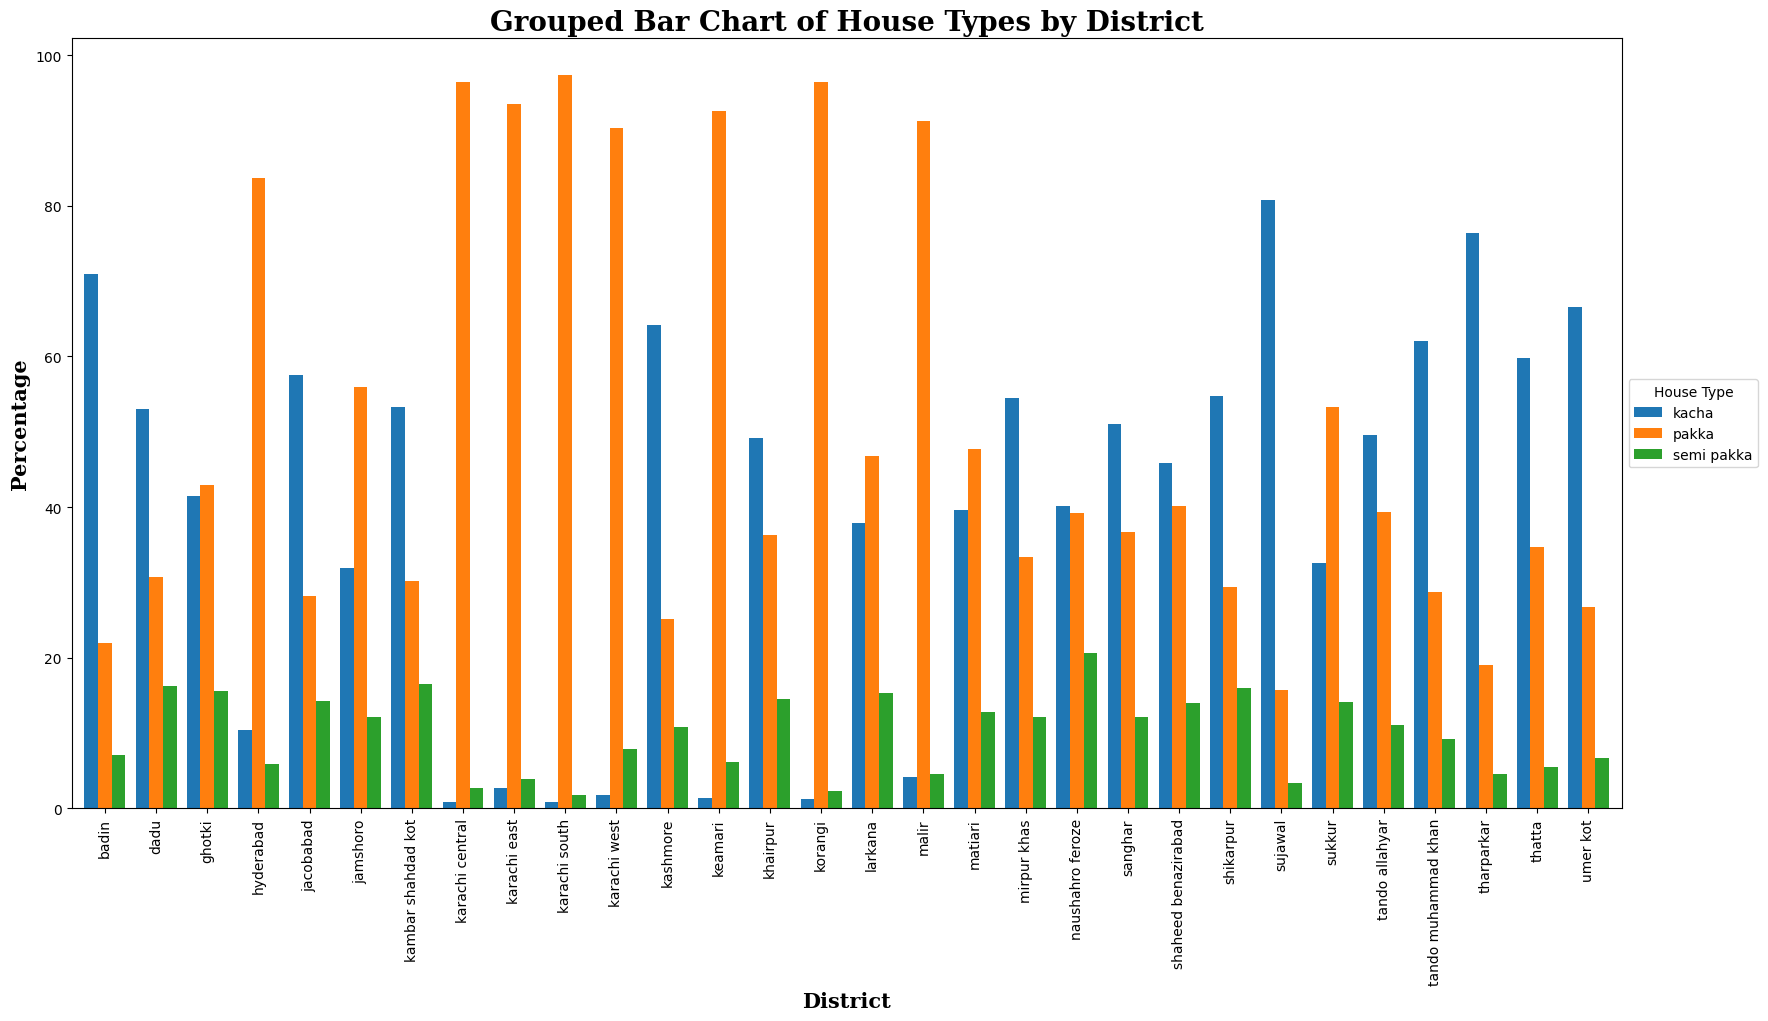
\includegraphics[width=\textwidth]{../Figures/Figure06.png}
    \caption{Distribution of housing infrastructure across different districts of Sindh.}
    \label{fig:fig5}
\end{figure}

\noindent Figure \ref{fig:fig5} shows the division of different housing types for different districts of the province. The main districts in focus will be the sub-districts of Karachi to understands if the housing infrastructure is better in Karachi due to it being one of the biggest city's in the country. 

\vspace{0.5cm}

\noindent It is interesting to observe that the seven sub-districts of Karachi have one of the \textit{best} housing infrastrucutre in the province with \textit{pakka} type of housing having the lime share of housing infrastructure in the city. Studies and analysis carried out in the past have also attributed housing infrastructure to wealth. The better the housing infrastructure, the more wealthier the district is. This can be used to make the inference that Karachi is the wealthiest district of the province and the country due to its stable housing infrastructure, as evident through its \textit{pakka} housing infrastructure.

\vspace{0.5cm}

\noindent The highest number of \textit{kacha} housing infrastructure is observed in the district of Sujawal, with the second highest \textit{kacha} housing infrastructure being in the district of Tharparkar, with Badin coming up as the third highest district with \textit{kacha} housing infrastructure.

\begin{figure}[H]
    \centering
    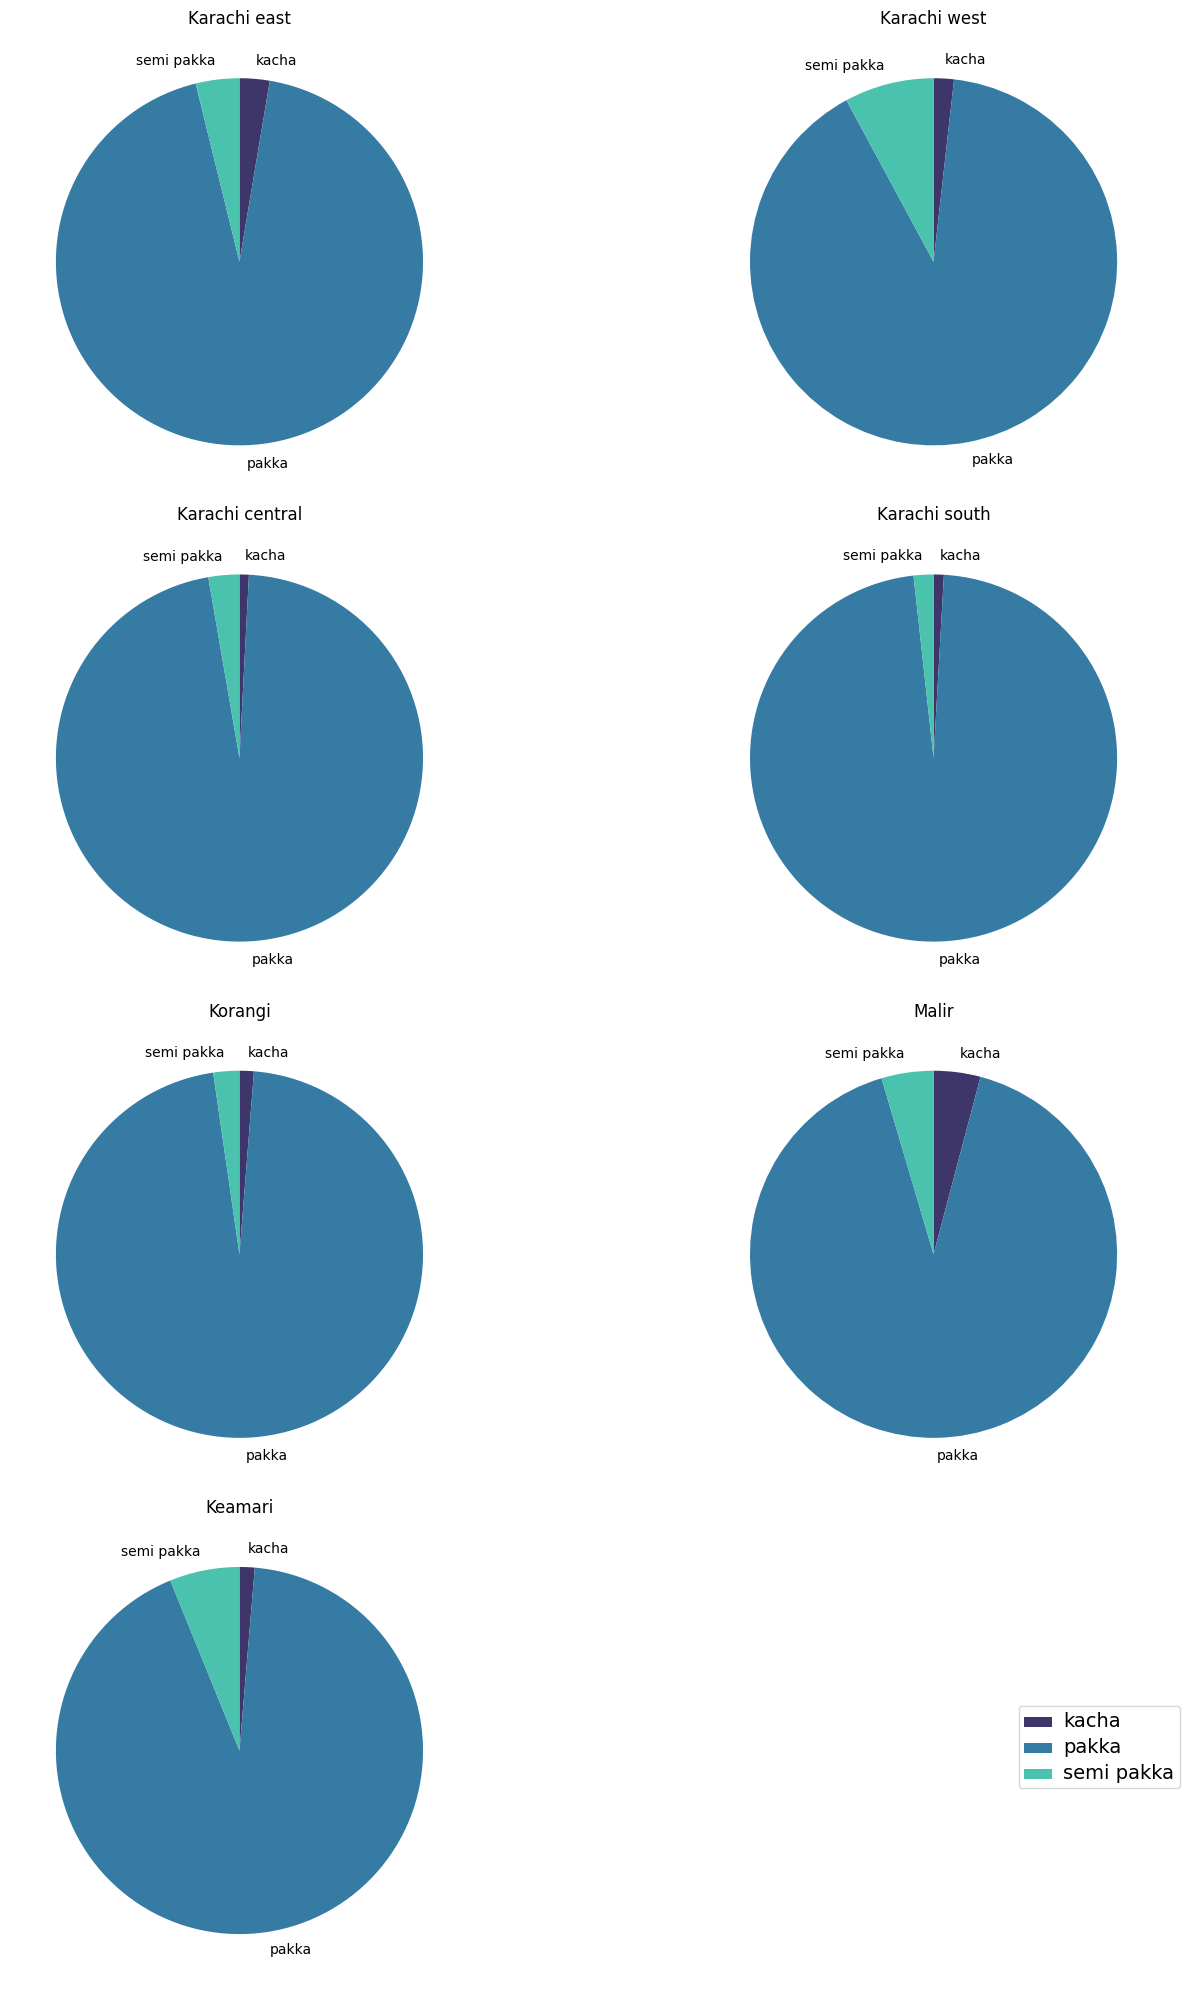
\includegraphics[width=0.7\textwidth]{../Figures/Figure07.png}
    \caption{Distribution of housing infrastructure across the seven sub-districts of Karachi.}
    \label{fig:fig6}
\end{figure}

\noindent Figure \ref{fig:fig6} further shed light on the housing infrastructure distribution in the sub-districts of Karachi where \textit{pakka} households dominate the other types of housing infrastructure.

\section*{Conclusion}

\noindent The analysis of the population of different districts of Sindh highlights the stark contrast between the most populated and largest districts of the province, the landmass of a district has no bearing on the population of that district. The population of the district largely depends on the number of opportunities, safety, security, and infrastructure that the district provides.

\vspace{0.5cm}

\noindent Karachi, being the economic hub of the country, has the highest population density in the province. The housing infrastructure of Karachi is also one of the best in the province, with the majority of the housing infrastructure being of the \textit{pakka} type. The average household size of the province is 5.53, with 13 out of 30 districts having an average household size greater than the provincial average.

\bibliographystyle{unsrt}
\bibliography{references}

\end{document}
